\documentclass[american,titlepage]{ntnuthesis} % TODO: Remove titlepage

\title{Computer Science, Specialization Project}
\shorttitle{Specialization Project}
\author{Aksel Lunde Aase \and Mathias Wold}
\shortauthor{A. L. Aase \and M. Wold}
\date{\today}

\addbibresource{thesis.bib}


% From https://www.overleaf.com/learn/latex/Glossaries

\makeglossaries % Prepare for adding glossary entries


\newglossaryentry{latex}
{
        name=latex,
        description={Is a mark up language specially suited for
scientific documents}
}

\newglossaryentry{bibliography}
{
        name=bibliography,
        plural=bibliographies,
        description={A list of the books referred to in a scholarly work,
typically printed as an appendix}
}

\newglossaryentry{maths}
{
    name=mathematics,
    description={Mathematics is what mathematicians do}
}


% --------------------
% ----- Acronyms -----
% --------------------

\newacronym{naplab}{NAPLab}{NTNU Autonomous Perception Laboratory}
\newacronym{carla}{CARLA}{Car Learning to Act}
\newacronym{lidar}{LIDAR}{Light Detection and Ranging}
 % add glossary and acronym lists before document

\begin{document}

\chapter*{Abstract}
The field of autonomous driving has seen great progress in recent years, but large-scale deployment of fully self-driving vehicles is still not currently present. Studies show that road traffic injuries are the main cause of death for people aged 5-29 worldwide, and that human driving errors are the cause of 92 \% of road accidents \cite{WHO-road-safety-report, towards-connected-autonomous-driving}. Self-driving vehicles could help reduce these accidents.

Motivated by this we will in this specialization project investigate a state-of-the-art model in the open-source autonomous driving simulator CARLA \cite{introducing-carla-paper}. More specifically we will look at a model proposed by \textcite{transfuser-pami} called TransFuser, which is one of the top performers on the CARLA Leaderboard \cite{carla-leaderboard}. The goal of this project is to set up CARLA on our own hardware and use it to train and evaluate TransFuser locally. This knowledge will then serve as a basis for our master thesis.

TransFuser is an end-to-end model for autonomous driving utilizing behaviour cloning to reach safe point-to-point navigation in an urban setting. We use TransFuser's included benchmark to experiment with three different model setups locally.
%This is done in an containerized environment to ensure comparability. 
Our results show worse driving score than originally reported by TransFuser on the CARLA Leaderboard. One possible culprit is that we used the wrong vehicle type for training and evaluation, which was a result of upgrading the TransFuser code to the latest CARLA version.
This upgrade could also have caused other unintended consequences.

Even with these results we show that training a custom TransFuser agent and evaluating it on the latest CARLA version is possible on our own hardware. We have developed and documented tooling which will be useful in future experiments. Finally, we include multiple suggestions of future work based on the knowledge gained in this specialization project.


\chapter*{Sammendrag}

TODO

\tableofcontents
% \listoffigures
% \listoftables
% \lstlistoflistings

\printglossary[type=\acronymtype] % Print acronyms
\printglossary                    % Print glossary

\chapter{Introduction}

\section{Background and Motivation}
The field of autonomous driving has seen rapid progress since the first computer controlled self-driving car was released in 1986 \cite{AV-history}. With a top speed of 32 km/h, the modified Chevrolet was capable of basic routing and obstacle avoidance. By 1995, prototype cars demonstrated lane keeping, cooperative driving and better vision of the surroundings. Today, these features are just some of the challenges faced when designing and creating fully autonomous vehicles, and large players in the industry such as Tesla and Google are publicly pushing the technology towards this common goal \cite{tesla-ai-day-2022, waymo-cvpr-2022}. An issue brief published by the Environmental and Energy Study Institute from last year suggests that half of the newly produced vehicles could be fully autonomous by 2050, and half of all vehicles by 2060 \cite{eesi-av-climate-solution}. Still, large-scale deployment of fully self-driving vehicles is not currently present.

%As the CEO of Tesla points out, the main challenge with autonomous driving is its root in the real world \cite{elon-musk-tweet-lol}. To remedy this, attempts of autonomous driving simplifies the environment in some way. For example, the World on Rails model assumes that "[...] the world is on rails, meaning that neither the agent nor it actions influence the environment" \cite{world-on-rails-paper}. Such assumptions and simplifications must be addressed before 

The United Nations Economic Commission for Europe (UNECE) publishes every two years statistics of road traffic accidents in Europe and North America \cite{UNECE-traffic-accidents-2021}. Their latest release show that almost 100,000 people died as a result of road traffic accidents, which equals to an average of 270 people per day. Together with the World Health Organization (WHO) they clearly state that road traffic injuries are the leading cause of deaths for people aged 5-29 worldwide \cite{WHO-road-safety-report}. This is a clear motivation for the development and deployment of autonomous vehicles. They could help reduce or even remove the effect of human driving errors, such as driver inattention, distractions, false assumptions and ignoring speed limits, which are the cause of around 92 \% of road accidents \cite{towards-connected-autonomous-driving}.

\todo{maybe add a paragraph about the environment and economical benefits of AVs}

% Other potential benefits of a deployment of autonomous vehicles include ... 

When building solutions for autonomous vehicles there are two choices for testing them: Either one uses real cars in real traffic, or one uses a realistic simulator. While the real world of course gives the most accurate results on a potential solution, a simulator can often be a good starting point. Not only are working with simulators instead of real cars much cheaper and more available to the research community, but it also has the advantage of iteration speed, data generation and safety. \acrfull{carla} is an open-source photo-realistic simulator for research on autonomous driving \cite{introducing-carla-paper}. It also includes an open leaderboard for evaluation of driving performance by autonomous agents in realistic traffic scenarios \cite{carla-leaderboard}.  

In this this specialization project we will investigate the TransFuser model \cite{transfuser-pami}, one of the top performers on the CARLA leaderboard. We will attempt to set up and run their custom evaluation on our available hardware, using both pre-trained and re-trained weights. Overall this project will give valuable insights and experience in preparation for our master thesis.


\begin{comment}
    
- How (connected) autonomous driving can mitigate traffic congestion, road safety, inefficient fuel consumption, etc. \cite{towards-connected-autonomous-driving}
- Mention why it is useful to experiment in a simulator? 
 --- Safety, easier to generate data, etc.

\end{comment}



\section{Goals and Research Questions}
Our research goal is ...

To reach this goal we will answer the following research questions:
\begin{itemize}
    \item \textbf{RQ1:} Hva er state-of-the-art (i et simulert miljø / i CARLA)?
    \item \textbf{RQ2:} Kan vi gjenskape state-of-the-art i CARLA?
    \item \textbf{RQ?:} Hvordan sette opp CARLA i IDUN(?)
    \item \textbf{RQ?:} Can we evaluate the TransFuser model using their pre-trained weights?
    \item \textbf{RQ?:} Can we evaluate the TransFuser model using our re-trained weights?
\end{itemize}


\section{Contributions}
As this specialization project is mainly a theoretical preparation for the master thesis, contributions are not in focus. Still, the project has produced the following contributions, which can be found on our GitHub:\footnote{https://github.com/orgs/aasewold/repositories}

\begin{itemize}
    \item An updated TransFuser code base which works on the newest version of CARLA (0.9.13).
    \item Python stub files for the CARLA Python API. These allow IDEs to show type hints and auto-completion for classes and methods imported from the CARLA package.
\end{itemize}


\section{Report Structure} % obs: thesis structure på masteren
This project report has the following structure:

\begin{description}
    \item[Chapter 1: Introduction] ...
    \item[Chapter 2: Background and Related Work] ...
    \item[Chapter 3: Methodology] ...
    \item[Chapter 4: Experiments and Results] ...
    \item[Chapter 5: Discussion] ...
    \item[Chapter 6: Conclusion and Future Work] ...
\end{description}

\chapter{Background and Related Work}
\label{chap:background}

Hva kan være interessant å skrive om her da hmm?

\begin{enumerate}

    
    \item NAP-lab vehicle
    
    \item Carla simulator
    \item Carla leaderboard
    
    \item Deep learning
    \begin{enumerate}
        \item Reinforcement learning and imitation learning
        \item Modular vs end-to-end approaches
    \end{enumerate}
    
    \item Existing models
    \begin{enumerate}
        \item Transfuser
        \item Interfuser
    \end{enumerate}
    
    \item Challenging tasks
    \begin{enumerate}
        \item Lane prediction
        \item
    \end{enumerate}
\end{enumerate}


\chapter{Methodology}
\label{chap:method}


% The method chapter should describe in detail which activities you undertake to answer the research questions presented in the introduction, and why they were chosen. This includes detailed descriptions of experiments, surveys, computations, data analysis, statistical tests etc.

\section{Tools and Resources}
Beskrive VM, IDUN, etc


\section{Creating Python Stubs for CARLA (?)}


\section{Upgrading Transfuser to CARLA Version 0.9.13}


\section{Experiment 1: Reproducing the Results from Transfuser}
Eventuelt dele disse to inn i to separate experiments:

\subsection{Using a Pre-Trained Model}

\subsection{Training Our Own Model}
Nevne noe om datasettet


\section{Experiment 2: XXX}

\chapter{Experiments and Results}
\label{chap:results}

% The results chapter should simply present the results of applying the methods presented in the method chapter without further ado. This chapter will typically contain many graphs, tables, etc. Sometimes it is natural to discuss the results as they are presented, combining them into a "Results and Discussion" chapter, but more often they are kept separate.

\section{Experiment 1: Evaluating TransFuser with pre-trained parameters}

The results from experiment 1 are shown in \autoref{tab:results:exp1}.

\begin{table}[]
    \centering
    \begin{tabular}{c|c}
        \textbf{Metric} & \textbf{Result} \\ \hline
        crashes & 1
    \end{tabular}
    \caption{Results from experiment 1.}
    \label{tab:results:exp1}
\end{table}


\section{Experiment 2: Evaluating TransFuser with re-trained parameters}

The results from experiment 2 are shown in \autoref{tab:results:exp2}.

\begin{table}[]
    \centering
    \begin{tabular}{c|c}
        \textbf{Metric} & \textbf{Result} \\ \hline
        crashes & 2 \\ \hline
        driving on sidewalk & yes
    \end{tabular}
    \caption{Results from experiment 2.}
    \label{tab:results:exp2}
\end{table}

\chapter{Discussion}
\label{chap:discussion}

\todo[inline]{burde kanskje bytta ut Leaderboard-tallene med Longest6-tallene fra TransFuser-paperet heller?}
% ^ er sikkert ikke så nøye, men synes ikke det siden vi nå rereferer til Leaderboard flere steder

\begin{table}[]
    \centering
    \begin{tabular}{|c|c|c|c|c|}
        \hline
        \textbf{Metric} & \textbf{Leaderboard} & \textbf{Exp. 1} & \textbf{Exp. 2} & \textbf{Exp. 3} \\ \hline
        Routes completed &
            36 / 36 &   30 / 36 &   30 / 36 & 30 / 36 \\ \hline
        Driving score &
            61.18   &   6.84\%  &   4.27\%  &   1.00\%  \\ \hline
        Route completion &
            86.7    &   82.3\%  &   63.6\%  &   3.63\%  \\ \hline
        Infraction penalty &
            0.710    &  0.130   &  0.170    &   0.308   \\ \hline
        Collisions with pedestrians &
            0.04    &   0.085   &   0.10    &   0.0     \\ \hline
        Collisions with vehicles &
            0.81    &   7.3     &   9.2     &  46.1     \\ \hline
        Collisions with layout &
            0.01    &   0.37    &   0.49    &  30.0     \\ \hline
        Red light infractions &
            0.05    &   0.085   &   0.070   &   0.73    \\ \hline
        Stop sign infractions &
            0.00    &   0.51    &   0.38    &   0.0     \\ \hline
        Off-road infractions &
            0.23    &   0.37    &   3.0     &  41.4     \\ \hline
        Route deviations &
            0.00    &   0       &   0.035   &   0.0     \\ \hline
        Route timeouts &
            0.01    &   0.28    &   0.21    &   2.19    \\ \hline
        Agent blocked &
            0.43    &   0.20    &   0.45    &  19.74    \\ \hline
    \end{tabular}
    \caption{Comparison of all experimental results.}
    \label{tab:discussion:comparison}
\end{table}

As can be seen from \cref{tab:discussion:comparison},
we observe worse results for all our experiments
than what TransFuser achieves on the online CARLA Leaderboard.
Though the Leaderboard evaluations are performed on a different, larger set of routes,
we can still conclude that driving performance is drastically reduced in our experiments.

One possible culprit is the use of the Tesla Model 3 instead of the Lincoln MKZ 2017 vehicle during evaluation.
This causes there to be a mismatch between the training data and evaluation data,
which could cause severe issues depending on how well the model generalizes to new data.
Both driving dynamics and vehicle collision box size could be changed between these vehicles,
possibly causing the observed increase in collision rates.
There could also be other factors such as a difference in height between the vehicles,
which would cause the cameras to record input images from a different point of view.
If the model correlates an object's vertical position in the input image
with its depth in the scene,
this could cause the model to incorrectly calculate the distance to other vehicles,
which could explain the observed results.

The reason for the vehicle replacement is that the intended vehicle
had changed its vehicle identifier
from \texttt{vehicle.lincoln.mkz2017}
to \texttt{vehicle.lincoln.mkz\_2017}
between CARLA version 0.9.10 and 0.9.13,
which we did not detect in our transition.
Thus the evaluation scripts failed to load the vehicle and instead used a fallback vehicle.
Future experiments should therefore investigate the performance difference of using the corrected vehicle identifier.

The CARLA version upgrade may also have caused other unintended consequences.
While we have not investigated these in further detail,
there is a possibility that there are slight rendering differences between the versions,
such as modified lightning, camera distortion model, weather, or 3D models.
This could cause the training dataset (which was generated on version 0.9.10)
to be obsolete and inadequate for driving well on version 0.9.13.
Expanding on this,
there could be other differences unrelated to graphics too,
for instance vehicle dynamics and handling.
We therefore recommend that future research generate a new dataset using CARLA version 0.9.13
to ensure compatibility.
An option then is to generate data from multiple different vehicles,
as this can help the model generalize to different vehicles and point of views.

It is also interesting that the ensemble in experiment 3 performed so poorly.
Given that the same method is used to evaluate the ensemble in experiment 1,
we find it unlikely that the implementation is to blame.
This indicates that the two additional custom-trained sets of weights used in the ensemble are the culprit,
thus these need to be evaluated individually to investigate if this is simply a result of poor training results.
If so, it would be interesting to perform additional training runs
to analyze the distribution of evaluation performance.



\chapter{Conclusion and Future Work}
\label{chap:conclusion}

%The conclusion chapter is usually quite short - a paragraph or two - mainly summarising what was achieved in the project. It should answer the claim part of the introduction. It should also say something about what comes next ("future work").

While the results are not entirely satisfying,
showing much lower performance than expected,
the experiments have still proven that training a custom TransFuser agent
and evaluating it on CARLA version 0.9.13
is possible on the available hardware.
The knowledge from running the experiments
have resulted in a well-documented method,
as well as multiple points to improve upon in the future.

We are satisfied with the development of the Carlo client
that assists in inspecting the driving performance of evaluation runs while they are active.
The containerization and tooling developed to enable the simulator to run on Idun
will also provide useful in future experiments.
Using the Idun cluster,
multiple experiments and evaluations can be performed in parallel,
significantly speeding up research.
Additionally, using the Idun cluster enables entirely new methods of compute-intensive learning
such as Direct Behaviour Learning and Reinforcement Learning,
both of which are intractable to execute in a reasonable time frame without opportunities for parallel training.


\section{Future Work}

During this research,
multiple ideas for improvement and future work have materialized.
Work remains to finish the transition to CARLA version 0.9.13,
specifically regarding the use of the Lincoln MKZ 2017 vehicle,
and generation of a new dataset with the correct simulator version.
It is also unclear why the custom-trained ensemble performed so poorly,
to investigate this issue the three constituent models should be evaluated individually.

As for possible beyond-baseline improvements,
this can be achieved in multiple ways.
Here we categorize the improvements based on their domain,
specifically whether they change the:
dataset,
learning algorithm,
agent itself,
or the simulator.

\subsection{Improvements to the dataset}

In addition to recreating the dataset using CARLA version 0.9.13,
there are other improvements that could be made to the dataset.
One of which is creating the dataset using multiple different vehicles
so that it contains data from different points of view
and learns to generalize better over its input data and different vehicle dynamics.

The simulator also supports two different rendering quality modes, Low and Epic.
To further increase the variance of the dataset,
data could be generated using both quality modes instead of just one.


\subsection{Improvements to the learning algorithm}

Previously discussed is the concept of Direct Policy Learning,
which could increase the generalizability of the model
by effectively making the training dataset more varied.
This would require implementing a new training loop which distributes
training across multiple nodes on the Idun cluster,
and which synchronizes additions to the dataset between the nodes while running.

Another, simpler, approach to this is to first train TransFuser on the original dataset using Behavioural Cloning,
then perform multiple model roll-outs to generate a new dataset using the model's state distribution,
and finally fine-tune the model on this new dataset.
This brings some of the benefits from Direct Policy Learning such as mitigating the Distribution Shift problem,
while being able to re-use the existing BC training methodology.


\subsection{Improvements to the agent}

During our experiments we noticed multiple issues with the agent's behaviour,
such as colliding with the vehicle in front,
driving on the pavement in right-turns,
and simply standing still with no obstacles or red light in sight.
We are curious about the agent's reasoning in these cases,
and believe that adding a new output head to the model that produces a one-hot encoded vector of reasons
could improve the explainability of the model.
The vector could for instance contain cells for
"Stopped because of red light",
"Turning right because the road turns right",
and "Changing lane to the left because I'm taking turning left in the intersection".
By extending the expert agent and dataset generation method
we could produce labeled data for this reason vector for the expert's decisions,
and then train TransFuser to output its own reasoning.

Another more radical approach is to separate the model into two sub-models,
a planner and an executor.
Both models would take as input the same data TransFuser already consumes,
but produce different output.
The planner outputs a command vector similar to the reason vector just explained,
which is used as additional input to the executor to condition it on a specific command.
The executor then produces output in the same format TransFuser does.
This latent command vector increases the explainability of the model
due to being interpretable,
and could enable external input to the model like
"keep left", "drive slowly", and "follow the car in front".

Yet another approach is to introduce a persistent hidden state vector
to let the model keep some memory of the immediate previous states,
turning the model into a recurrent neural network.
However this needs adjustment to the data-generation approach,
as data is currently sampled at random ticks while driving through the simulator.
To enable the model to utilize the state vector,
we would need data that covers multiple consecutive ticks in the simulator.
This would require generating a much larger dataset to keep the same variability,
since very little of the scene actually changes from tick to tick.


\subsection{Improvements to the simulator}

% snow poles her? og litt om snø generelt?


% \subsection{Using Snow Poles for Detecting Snow Covered Roads}

 In Norway there is a established infrastructure around snow poles that assist human drivers during the winter months \cite{statens-vegvesen-handbok-111}. Their purpose is to mark the road outline when snow can make it hard for plow trucks and drives to see where road is. They normally placed on both sides of the road at a given interval, and have a reflective mark near the top. Knowing this, it would be interesting to find out whether snow poles can also assist autonomous cars in detecting snow covered roads. This is further motivated by multiple studies that highlight challenges for autonomous driving in adverse weather conditions \cite{impact-of-adverse-weather-conditions, Sensor-Fusion-Based-Semantic-Segmentation}, as these challenges need to be solved before cars can become fully autonomous in countries prone to these weather conditions.

Such a research project would require implementing a snow variant of a CARLA map, as this does currently not exist. This includes creating a new simulator asset in the form of a snow pole and placing instances of it in appropriate places around the map. Additionally it could be interesting to explore the effect of adding slippery roads and reduced sensory range due to snowy weather. CARLA thankfully supports both customizing maps and adding new assets \cite{carla-custom-maps, carla-custom-props}. When the snow map with snow poles are implemented, a new model would need to be trained. The methods and results from this specialization project could be used as a starting point for creating new experiments comparing driving performance before and after adding snow poles and/or snowy weather conditions. % Note that if implementing a snow covered map proves to be difficult, one could also simply experiment on the effect of adding snow poles to the simulation. This would still result in useful insights in the effect of using snow poles to navigate roads.


\begin{comment}
\begin{enumerate}
    \item Fungerer Direct Policy Learning bedre enn Behavioural Cloning?
        \\ - eventuelt lage et nytt datasett som styres av den ferdigtrente modellen i stedet for ekspertagenten,
            men som likevel får labels av ekspertagenten. Kan da fintune TransFuser på det nye datasettet, eventuelt trene fra scratch med kombo av begge.

    \item Mulig å trene en Transition function som predicter future state?
        Ta outputen $Z$ og $Z'$ fra Transfuser backbonet for to states $s$ og $s'$ og action $a$
        Supervised learning for å lære $T: (Z, a) \rightarrow Z'$

    \item Mulig å trene en forklarings-funksjon som tar inn Z' og predicter hvorfor bilen gjør som den gjør
        \\ - venter på rødt lys/stoppskilt/??
        \\ - sakker ned pga ???
        \\ - speeder opp pga ???
        \\ - svinger (venstre? høyre?) fordi ??
        \\ - kjører i oppover/nedoverbakke
        \\ - er det biler i fila til venstre? høyre?
        \\ - er det motkommende bil?
        \\ - regner det? glatt?

    \item Recurrent Transfuser? Legge til en MLP som tar $(Z_{t-1}, Z) \rightarrow Z'$
        Nødvendig med nytt datasett da og ny trening. Må trene på konsistente episoder og resette state-vector hver gang man går over i en ny episode for at det skal matche inference-time miljøet. Evt. om vi kan ha treningssamples med alt fra 10ms til 2000ms mellom hvert tick, lærer den å takle det mon tro?

    \item Lage dataset med både low- og high-quality bilder
    
    \item Feature Pyramid Network attached to the ends of both the Image and BEV branches.
    
    \item Combine both Image and BEV outputs (with dropout to ensure the transformers are necessary for information sharing) through a big MLP and use the output as input to all the auxiliary tasks (instead of taking HD map directly from BEV for instance). Summary: bottleneck everything through a latent vector.
    
    \item Analyze class imbalance in the training data, for instance in the segmentation maps. Too much sky, road, ...?
    \begin{enumerate}
        \item Focal Loss or manual $\alpha$-scaling?
    \end{enumerate}
    
    \item Use the HD map for waypoint and route planning?
    \begin{enumerate}
        \item HD-map currently currently classifies into "road", "lane marking", and "other". Good enough?
        \item Use it to prevent driving on sidewalk
        \item Lane detection ...
    \end{enumerate}
\end{enumerate}
\end{comment}

\chapter*{\bibname}
\printbibliography[heading=none]

% % First paper

\begin{paper}{papers/landes1951scrutiny.pdf}{paper:scrutiny}
    Here, you may add a description of the paper, an illustration, or just give the bibliographic reference:
    \begin{quote}
        \fullcite{landes1951scrutiny}
    \end{quote}
    Or you may leave it empty, if you like.
\end{paper}

% Second paper etc.

\appendix
\chapter{Additional Material}
\label{app:additional}

Additional material that does not fit in the main thesis but may still be relevant to share, e.g., raw data from experiments and surveys, code listings, additional plots, pre-project reports, project agreements, contracts, logs etc., can be put in appendices. Simply issue the command \texttt{\textbackslash appendix} in the main \texttt{.tex} file, and make one chapter per appendix.

If the appendix is in the form of a ready-made PDF file, it should be supported by a small descriptive text, and included using the \texttt{pdfpages} package. To illustrate how it works, a standard project agreement (for the IE faculty at NTNU in Gjøvik) is attached here. You would probably want the included PDF file to begin on an odd (right hand) page, which is achieved by using the \texttt{\textbackslash cleardoublepage} command immediately before the \texttt{\textbackslash includepdf[]\{\}} command. Use the option \texttt{[pages=-]} to include all pages of the PDF document, or, e.g., \texttt{[pages=2-4]} to include only the given page range.

\cleardoublepage
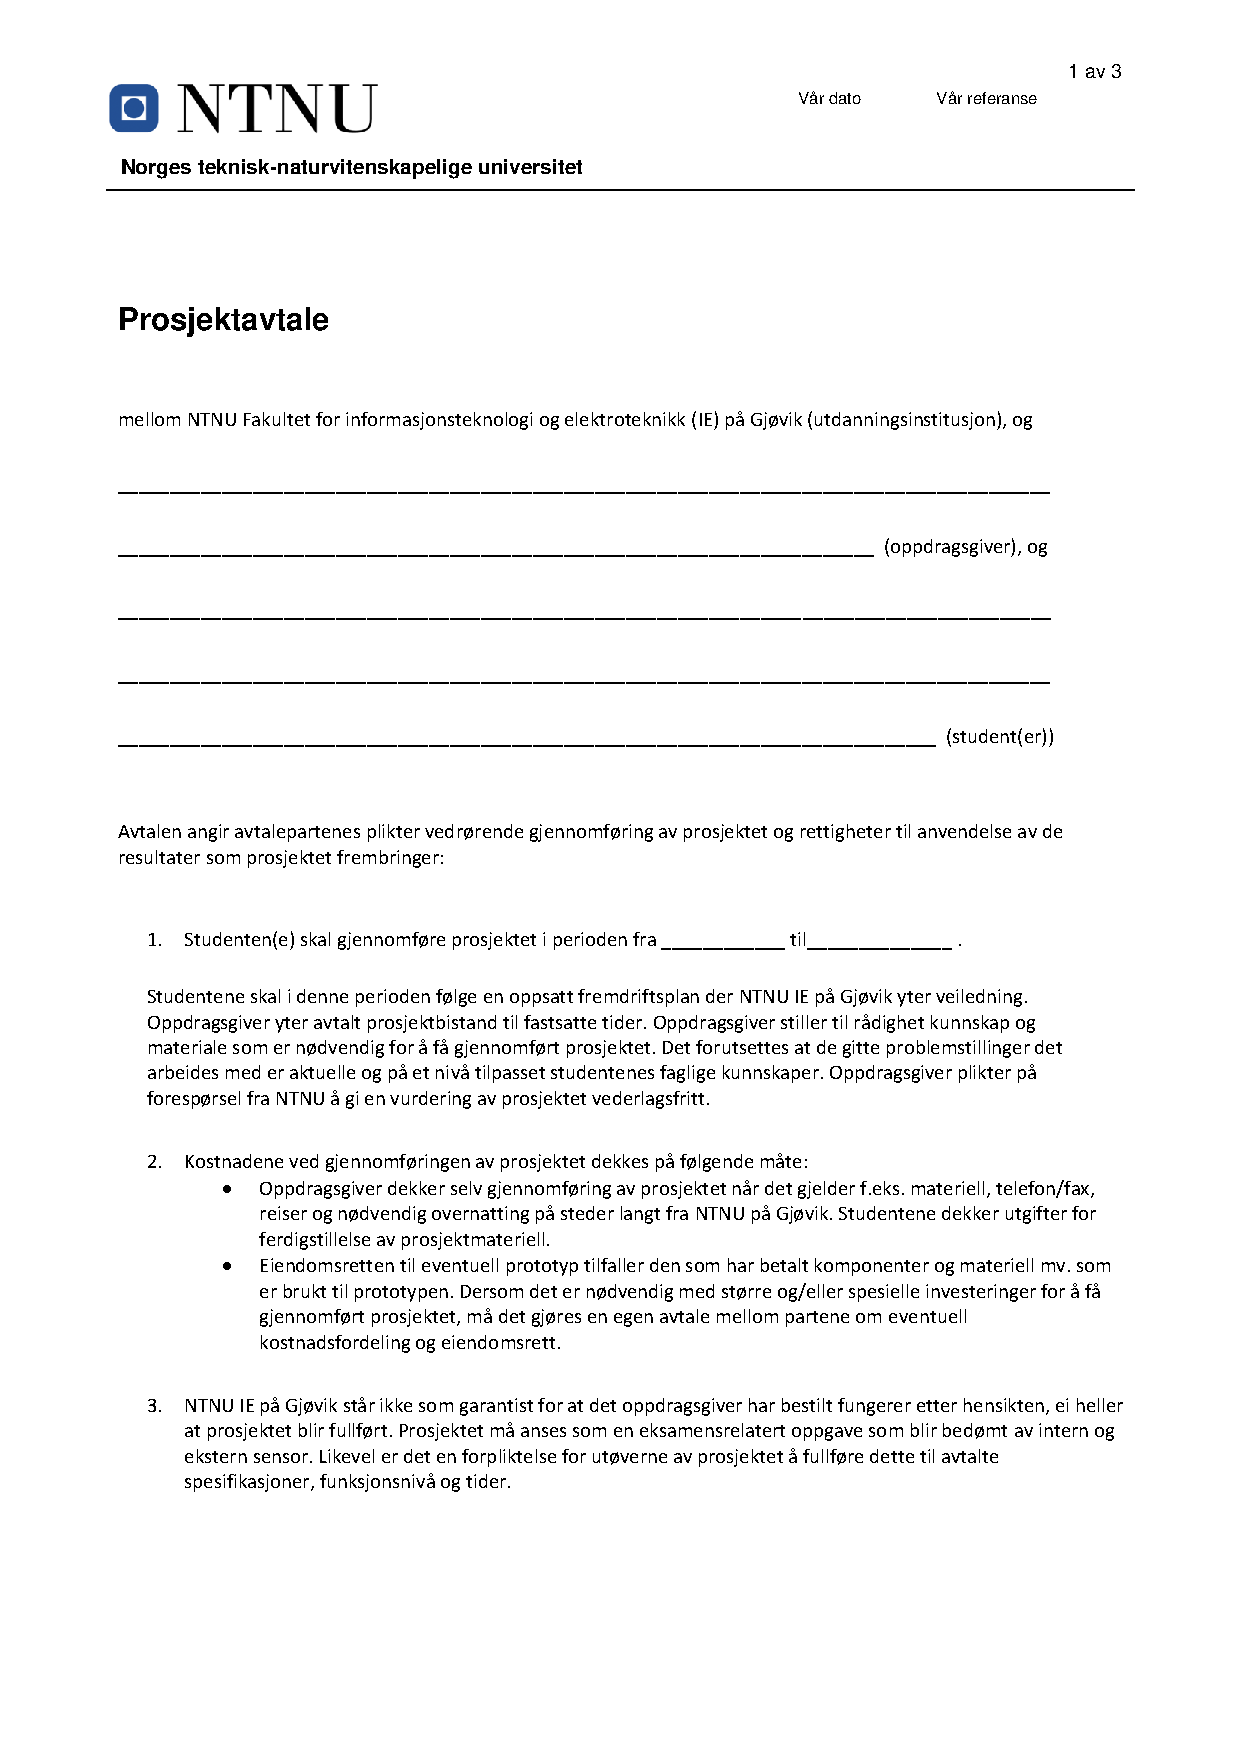
\includepdf[pages=-]{appendices/NTNUProsjektavtale.pdf}

\end{document}
